\documentclass[12pt,a4paper]{article}
%\usepackage[utf8]{inputenc}
%\usepackage[portuguese]{babel}
\usepackage{xcolor}
\usepackage[linesnumbered,ruled,vlined]{algorithm2e}
\usepackage{caption}
\usepackage{float} % to use [H]
\usepackage[skip=0.5ex]{subcaption}

\interfootnotelinepenalty=10000 % restrict is to one page
\SetKwInput{KwInput}{Input}                % Set the Input
\SetKwInput{KwOutput}{Output}              % set the Output
%%% Coloring the comment as blue
\newcommand\mycommfont[1]{\footnotesize\ttfamily\textcolor{blue}{#1}}
\SetCommentSty{mycommfont}

\newcommand\abs[1]{\left\lvert#1\right\rvert}

\usepackage{amsfonts}

\newcommand{\trans}{\mathsf{T}}
\newcommand{\hermit}{\mathsf{H}}
\newcommand{\mc}[1]{\ensuremath{\mathcal{#1}}}
\newcommand{\mbb}[1]{\ensuremath{\mathbb{#1}}}
\newcommand{\Natural}{\mathbb{N}}
\newcommand{\Integer}{\mathbb{Z}}
\newcommand{\Irrational}{\mathbb{I}}
\newcommand{\Rational}{\mathbb{Q}}
\newcommand{\Real}{\mathbb{R}}
\newcommand{\Complex}{\mathbb{C}}
\newcommand{\obs}[1]{\textcolor{red}{(#1)}}
\newcommand{\sizecorr}[1]{\makebox[0cm]{\phantom{$\displaystyle #1$}}} % Used to seize the height of equation
%\newcommand{\iff}{\mbox{$\Longleftrightarrow$}}    % biimplication
% \newcommand{\and}{\wedge}
% \newcommand{\or}{\vee}
\newcommand*\diff{\mathop{}\!\mathrm{d}}
\newcommand*\Diff[1]{\mathop{}\!\mathrm{d^#1}}
\newcommand{\ensureoperation}{\negmedspace {}} % To ensure that a new line symbol is an operation instead of a sign

\usepackage{amsmath, amsfonts, amssymb}
\usepackage{graphicx}
\usepackage{float}
\usepackage[utf8]{inputenc} % Permite utilizar caracteres especiais: Ex: ç á à...
\usepackage[onehalfspacing]{setspace} % Espaçamento de 1,5
\usepackage{cabecalho}
\usepackage{multirow}
\usepackage[lmargin=3cm, tmargin=3cm, rmargin=2cm, bmargin=2cm]{geometry}
\usepackage{indentfirst}
% \usepackage[brazilian]{babel} % Traduzir para PT-BR
\usepackage{IEEEtrantools}

\begin{document}
\initcab{Universidade Federal do Ceará}{Inteligência Computacional}{Guilherme Barreto and Ajalmar}{519024}{\today}{Homework 03 - Metaheuristic}

In the optimization theory field, a metaheuristic is a problem-independent algorithmic methodology that provides a set of guidelines to develop a problem-dependent heuristic solution, providing sufficiently good results to a given optimization problem \cite{ABDELBASSET2018185}. Heuristic solutions are attractive when
\begin{itemize}
    \item The classical methods are too slow or fail in finding the global solution.
    \item The computational capacity is limited or unaffordable.
    \item There is incomplete or imperfect information.
\end{itemize}

The main drawback is that we cannot guarantee that the global optimal solution will be found by using heuristic methods since they only sample a subset of the solution space. This subset is called search space, and a partial search algorithm is utilized to find a heuristic solution. That being said, the main goal of the metaheuristic is to efficiently explore the search space in order to find a near-optimal solution for nonspecific problems.

In this homework, we will focus on particle swarm optimization (PSO), which is a method from the natured-inspired metaheuristic branch.

Let us define
\begin{align}
    \mathbf{x}_i^{(m)} = \begin{bmatrix}
        x_1^{(m)} & x_2^{(m)} & \cdots & x_D^{(m)}
    \end{bmatrix}^\trans \in \Real^D,
\end{align}
and
\begin{align}
    \mathbf{v}_i^{(m)} = \begin{bmatrix}
        v_1^{(m)} & v_2^{(m)} & \cdots & v_D^{(m)}
    \end{bmatrix}^\trans \in \Real^D,
\end{align}
as the \(i\)th particle position and its velocity at the instant \(m\), respectively, where \(D\) is the length of the solution and \(i \in \left\{ 1, 2, \cdots, I \right\}\). The PSO algorithm that explores both the cognitive component of the individual experience and the social component to update \(\mathbf{x}_i^{(m)}\) and \(\mathbf{v}_i^{(m)}\). The recursive equations are given by
\begin{align}
    \mathbf{v}_i^{(m+1)} = w\mathbf{v}_i^{(m)} + c_1 \mathbf{r}_1 \odot \left( \mathbf{p}_i^{(m)} - \mathbf{x}_i^{(m)} \right) + c_2 \mathbf{r}_2 \odot \left( \mathbf{g}^{(m)} - \mathbf{x}_i^{(m)} \right)
    \label{eq:vi-update}
\end{align}
and
\begin{align}
    \mathbf{x}_i^{(m+1)} = \mathbf{x}_i^{(m)} + \mathbf{v}_i^{(m+1)},
    \label{eq:xi-update}
\end{align}
where \(w\) is the inertia parameter, \(c_1\) and \(c_2\) are the coefficient accelerators, \(\mathbf{r}_1\) and \(\mathbf{r}_2\) are constant vectors whose values come from the sampling of a random process with a uniform distribution between 0 and 1, \(\mathbf{p}_i^{(m)}\) is the best position of the \(i\)th particle, \(\mathbf{g}^{(m)}\) is the best global position, and \(\odot\) denotes the Hadamard operator.

Vectors \(\mathbf{x}_i^{(m+1)}\) and \(\mathbf{v}_i^{(m+1)}\) are limited to the range \([\mathbf{x}_l, \mathbf{x}_u]\) and \([-\abs{\mathbf{x}_u-\mathbf{x}_l}, \abs{\mathbf{x}_u-\mathbf{x}_l}]\), respectively, where \(\mathbf{x}_l\) and \(\mathbf{x}_u\) contains the elements of the lower and upper bounds of the search space.

For this homework, we will use the data set shown in Figure \ref{fig:scatter-plot}.
\begin{figure}[H]
    \centering
    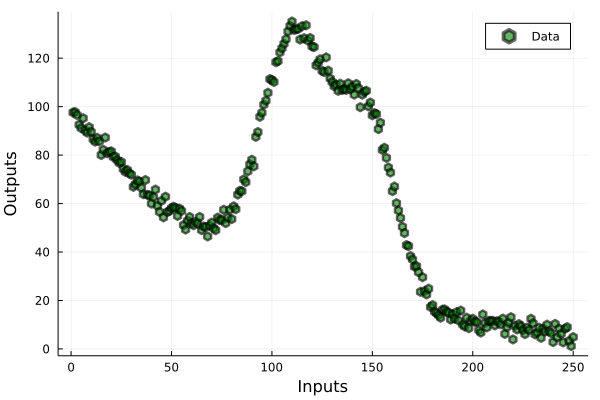
\includegraphics[scale=0.35]{../../TC1 - Sistemas Fuzzy para Regressão Não Linear/figs/OLS-by-parts/scatterplot.png}
    \caption{Scatterplot of the residuals.}
    \label{fig:scatter-plot}
\end{figure}

The goal is to find the coefficients of the \(k\)-order polynomial function, that is,
\begin{align}
    y(n) = a_0 + a_1 x(n) + a_2 x^2(n) + \cdots + a_k x^k(n),
\end{align}
where \(x(n)\) is the \(n\)th dataset sample and \(k=6\)\footnote{The value of \(k=6\) was defined based on the reasonable results achieved by the polynomial regressor.} is the polynomial function order. Hence
 \begin{align}
    \mathbf{x}_i^{(m)} = \begin{bmatrix}
        a_0^{(m)} & a_1^{(m)} & \cdots & a_k^{(m)}
    \end{bmatrix}^\trans \in \Real^{k+1}.
\end{align}
The best individual and global positions are defined based on a cost function, which is defined by the problem. The cost or objective function of this problem is given by
\begin{align}
    J_i^{(m)} = \sum_{n=1}^{N} e_i^2 (n),
\end{align}
where \(N\) is the length of the dataset and \(e_i(n) = y(n) - \hat{y}_i(n) \) is the residual error, being \(\hat{y}_i(n)\) the output value of the polynomial curve when it is used \(\mathbf{x}_i^{(m)}\) as the set of parameters.

The Algorithm \ref{alg:global-random-search} summarizes the PSO method, where the stop criteria is iterating over the dataset \(N_i\) times. Moreover, the inertia parameter, \(w\), is initialized at a high value (\(\simeq 0.9\)) and is gradually decreased to its minimum value (\(\simeq 0.4\)), making the GRS algorithm vary from exploring\footnote{The exploration phase where the algorithm tries to follow different paths in order to explore and space search and in better solutions.} to exploiting\footnote{Is the phase where the algorithm becomes more conservative in the sense that it tends to follow the same direction.}, respectively. The final output is the global best solution found by the swarm.

\begin{algorithm}[H]
    \DontPrintSemicolon
      
      \KwInput{\(D, J(\cdot), I, N_i, c_1, c_2\)}
      \KwOutput{\(\mathbf{g}^{(m)}\)}
      \KwData{\(\left\{ x(n) \right\}_{n=0}^N\)}
      
      \(\mathbf{x}_i^{(m)}, \mathbf{v}_i^{(m)}, w \leftarrow \) Initialize

      \(\mathbf{p}_i^{(m)} \leftarrow \mathbf{x}_i^{(m)}\)

      \ForAll{\(m \in \left\{ 1, , \cdots, N_i \right\}\)}{
        \ForAll{\(i \in \left\{ 1, , \cdots, I \right\}\)}{
            \(\mathbf{r}_1, \mathbf{r}_2 \leftarrow \) sample it from \(\sim U(0, 1)\)

            \(\mathbf{v}_i^{(m+1)} \leftarrow w\mathbf{v}_i^{(m)} + c_1 \mathbf{r}_1 \odot \left( \mathbf{p}_i^{(m)} - \mathbf{x}_i^{(m)} \right) + c_2 \mathbf{r}_2 \odot \left( \mathbf{g}^{(m)} - \mathbf{x}_i^{(m)} \right)\)

            \(\mathbf{v}_i^{(m+1)} \leftarrow\) limit it to \([-\abs{\mathbf{x}_u-\mathbf{x}_l}, \abs{\mathbf{x}_u-\mathbf{x}_l}]\)

            \(\mathbf{x}_i^{(m+1)} \leftarrow \mathbf{x}_i^{(m)} + \mathbf{v}_i^{(m+1)}\)

            \(\mathbf{x}_i^{(m+1)} \leftarrow\) limit it to \([\mathbf{x}_l, \mathbf{x}_u]\)

            \(J_i^{(m+1)} \leftarrow \sum_{n=1}^{N} e_i^2 (n)\)

            \eIf{\(J_i^{(m+1)} < J_i^{(m)}\)}{
                \(\mathbf{p}_i^{(m+1)} \leftarrow \mathbf{x}_i^{(m+1)}\)
                
            }{
                \(\mathbf{p}_i^{(m+1)} \leftarrow \mathbf{p}_i^{(m)}\)
            }

            \eIf{\(J_i^{(m+1)} < J_j^{(m)}\: \forall j \in \left\{ 1, 2, ..., I \right\}, j \neq i\)}{
                \(\mathbf{g}^{(m+1)} \leftarrow \mathbf{x}_i^{(m+1)}\)
                
            }{
                \(\mathbf{g}^{(m+1)} \leftarrow \mathbf{g}^{(m)}\)
            }
        }
      }
      \Return{\(\mathbf{g}^{(m)}\)}
    
    \caption{Particle Swarm Optimization}
    \label{alg:global-random-search}
\end{algorithm}

The same process was repeated \(M\) times. The result of the curve fitting is shown in Figure \ref{fig:heuristic-regression} for three independent realizations.

\begin{figure}[H]
    \centering
    \begin{subfigure}{0.6\textwidth}
        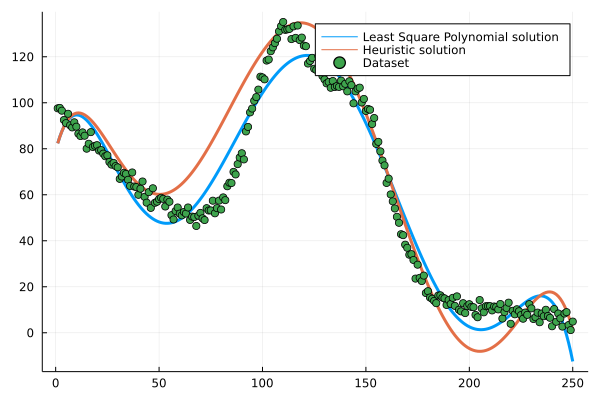
\includegraphics[width=\linewidth]{../figs/methaeuristic_regression_result1.png}
        \subcaption{First realization.}
        % \label{subfig:item2}
    \end{subfigure}
\end{figure}%
\begin{figure}[H]\ContinuedFloat
    \centering
    \begin{subfigure}{0.6\textwidth}
        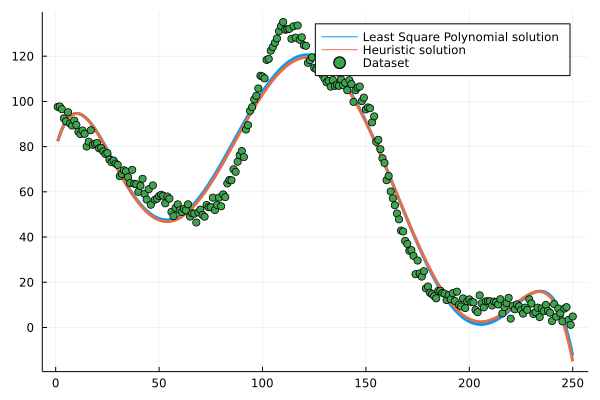
\includegraphics[width=\linewidth]{../figs/methaeuristic_regression_result2.png}
        \subcaption{Second realization.}
        % \label{subfig:item3}
    \end{subfigure}
\end{figure}    
\begin{figure}[H]\ContinuedFloat
    \centering
    \begin{subfigure}{0.6\textwidth}
        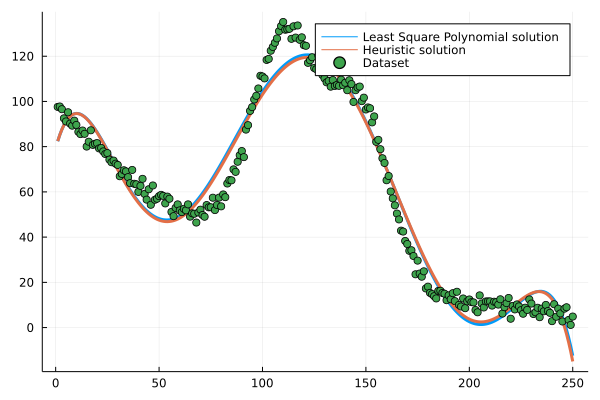
\includegraphics[width=\linewidth]{../figs/methaeuristic_regression_result3.png}
        \subcaption{Third realization.}
    \end{subfigure}
    \caption{result of the curve regression through PSO.}
    \label{fig:heuristic-regression}
\end{figure}

The value of the coefficients also varies with the independent realizations. Notwithstanding, these values are relatively close to the best solution. For comparison, the best solution is
\begin{align}
    \mathbf{x}_o = \begin{bmatrix}
        79.2057 \\ 3.44317 \\ -0.230983 \\ 0.0045354 \\ -3.70951.10^{-5} \\ 1.34374.10^{-7} \\ -1.79008.10^{-10}
    \end{bmatrix},
\end{align}
while the solution found by the PSO is
\begin{align}
    \mathbf{g} = \begin{bmatrix}
        79.2057 \\ 3.44607 \\ -0.221978 \\ 0.00442822 \\ -3.67436.10^{-5} \\ 1.34206.10^{-7} \\ -1.79343.10^{-10}
    \end{bmatrix}
\end{align}.

The Global Random Search (GRS), which is a nonnature-inspired metaheuristic technique, could achieve similar results, as shown in Figure \ref{fig:global-random-search-fit}.

\begin{figure}[H]
    \centering
    \begin{subfigure}{0.6\textwidth}
        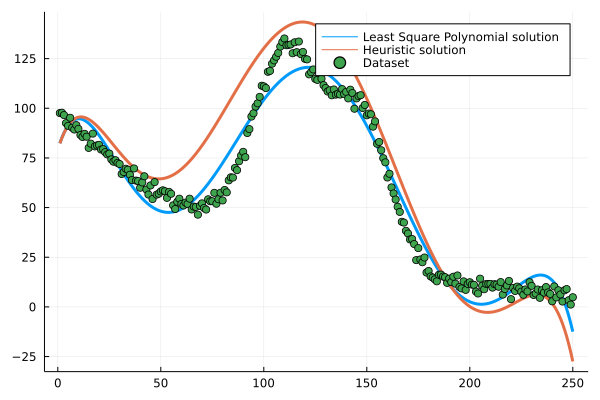
\includegraphics[width=\linewidth]{../figs/grs_regression_result1.png}
        \subcaption{First realization.}
        % \label{subfig:item2}
    \end{subfigure}
\end{figure}%
\begin{figure}[H]\ContinuedFloat
    \centering
    \begin{subfigure}{0.6\textwidth}
        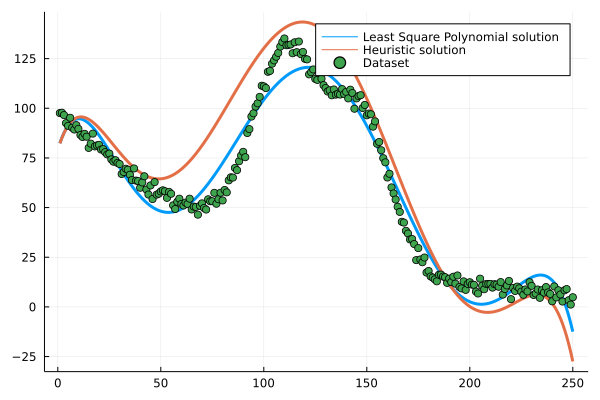
\includegraphics[width=\linewidth]{../figs/grs_regression_result2.png}
        \subcaption{Second realization.}
        % \label{subfig:item3}
    \end{subfigure}
\end{figure}    
\begin{figure}[H]\ContinuedFloat
    \centering
    \begin{subfigure}{0.6\textwidth}
        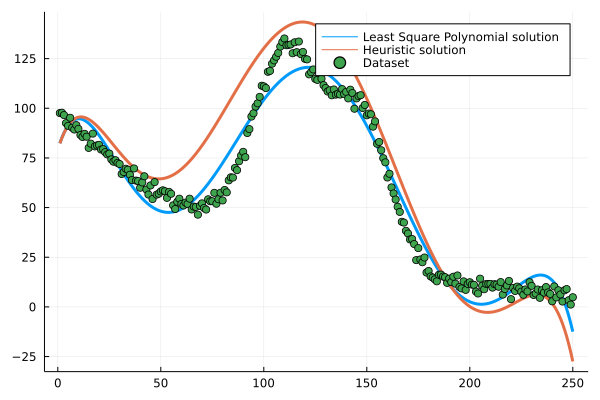
\includegraphics[width=\linewidth]{../figs/grs_regression_result3.png}
        \subcaption{Third realization.}
    \end{subfigure}
    \caption{result of the curve regression through GRS.}
    \label{fig:global-random-search-fit}
\end{figure}

Despite the good results, both PSO and GRS are very sensitive to the search space range. In other words, they only achieve reasonable results when the search space is very close to the best solution. Otherwise, the best solution can differ significantly from a reasonable result.

Although the PSO is much more costly than the GRS, the final results suggest that the swarm approach outperforms the individual random search method.

For the following cost function
\begin{align}
    J_i^{(m)} = \sum_{n=1}^{N} \abs{e_i (n)},
\end{align}

The results of the curve fitting are shown in Figure \ref{fig:heuristic-regression2}.

\begin{figure}[H]
    \centering
    \begin{subfigure}{0.6\textwidth}
        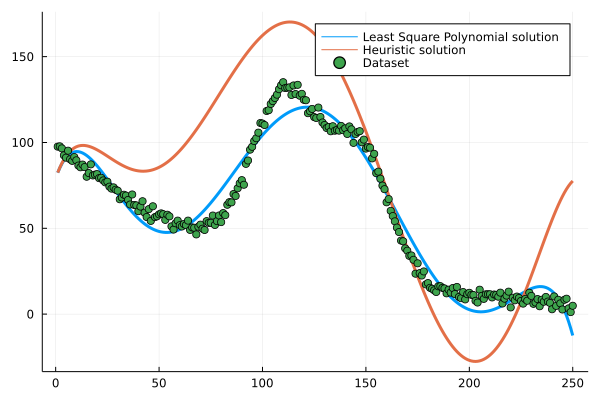
\includegraphics[width=\linewidth]{../figs/methaeuristic_regression_result1F.png}
        \subcaption{First realization.}
        % \label{subfig:item2}
    \end{subfigure}
\end{figure}%
\begin{figure}[H]\ContinuedFloat
    \centering
    \begin{subfigure}{0.6\textwidth}
        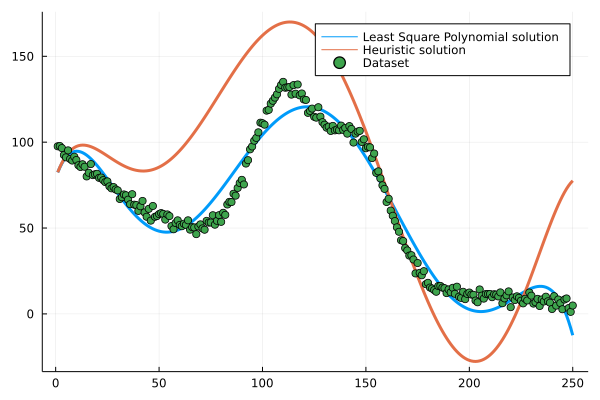
\includegraphics[width=\linewidth]{../figs/methaeuristic_regression_result2F.png}
        \subcaption{Second realization.}
        % \label{subfig:item3}
    \end{subfigure}
\end{figure}    
\begin{figure}[H]\ContinuedFloat
    \centering
    \begin{subfigure}{0.6\textwidth}
        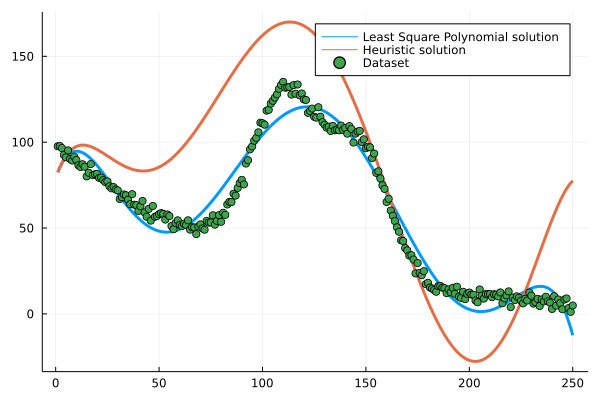
\includegraphics[width=\linewidth]{../figs/methaeuristic_regression_result3F.png}
        \subcaption{Third realization.}
    \end{subfigure}
    \caption{result of the curve regression through PSO.}
    \label{fig:heuristic-regression2}
\end{figure}

These results are significantly worse than the squared value.

\bibliography{ref.bib}
\bibliographystyle{ieeetr}

\end{document}